%
% Sample SBC book chapter
%
% This is a public-domain file.
%

\documentclass{SBCbookchapter}
\usepackage[utf8]{inputenc}
\usepackage[T1]{fontenc}
\usepackage{lmodern}
\usepackage[brazilian,english]{babel}
\usepackage{graphicx}
\usepackage{natbib}
\usepackage{listings}
\usepackage{color}
\usepackage{algorithm}
\usepackage{algorithmic}
\usepackage{amsmath}
\usepackage[round]{natbib}


\renewcommand{\algorithmicrequire}{\textbf{Input:}}
\renewcommand{\algorithmicensure}{\textbf{Output:}}
\renewcommand{\algorithmicif}{\textbf{se}}
\renewcommand{\algorithmicthen}{\textbf{então}}
\renewcommand{\algorithmicdo}{\textbf{faça}}
\renewcommand{\algorithmicend}{\textbf{fim}}
\renewcommand{\algorithmicfor}{\textbf{para}}

\definecolor{dkgreen}{rgb}{0,0.6,0}
\definecolor{gray}{rgb}{0.5,0.5,0.5}
\definecolor{mauve}{rgb}{0.58,0,0.82}


\lstdefinestyle{MySQLStyle}{
  frame=tb,
  language=SQL,
  aboveskip=3mm,
  belowskip=3mm,
  showstringspaces=false,
  columns=flexible,
  basicstyle={\small\ttfamily},
  numbers=none,
  numberstyle=\tiny\color{gray},
  keywordstyle=\color{blue},
  commentstyle=\color{dkgreen},
  stringstyle=\color{mauve},
  breaklines=true,
  breakatwhitespace=true,
  tabsize=3
}

\lstdefinestyle{MyPythonStyle}{
  frame=tb,
  language=Python,
  aboveskip=3mm,
  belowskip=3mm,
  showstringspaces=false,
  columns=flexible,
  basicstyle={\small\ttfamily},
  numbers=none,
  numberstyle=\tiny\color{gray},
  keywordstyle=\color{blue},
  commentstyle=\color{dkgreen},
  stringstyle=\color{mauve},
  breaklines=true,
  breakatwhitespace=true,
  tabsize=3
}

\lstset{language=Python,frame=tb}
\lstset{language=SQL,frame=ltrb}


\author{Victor Teixeira de Almeida e Vitor Alcântara Batista}
\title{Tecnologias para gerenciamento de dados na era do big data}

\begin{document}

\maketitle
\inputencoding{utf8}
\selectlanguage{brazilian}

\begin{abstract}
\begin{otherlanguage}{english}
This short course is an overview of big data management, and
intends to explore and diferentiate several recent technologies. A
classic problem of the database community will be used as a background for the 
examples given throughout this course: triangle counting on graphs. It's been 
initially chosen because of its frequent application in a real and practical problem: 
identifying the importance of individuals on social networks. 
Also, since it can be described by an algorithm that is simple to understand and 
yet complex to execute in terms of performance, the differences between technologies
in design and performance will be easily demonstrated. 
\end{otherlanguage}
\end{abstract}

\begin{resumo}
Este minicurso pretende explorar e diferenciar de forma introdutória diversas 
tecnologias recentes
para gerenciamento de dados na era do big data. Será utilizado como pano de fundo para os
exemplos um problema clássico da comunidade de bancos de dados: a contagem de triângulos
em grafos. Ele foi escolhido, inicialmente, por ser um problema atual e prático, frequentemente 
utilizado para identificar a importância de indivíduos em redes sociais. Além disso, por ser de
fácil representaçao e alta complexidade de execução, é possível demonstrar, através do seu uso, 
as diferenças entre as tecnologias em termos de expressividade e desempenho. 
\end{resumo}


\section{Introdução}

\section{Contagem de triângulos} 
\label{sec:triangulos}

Nesta seção, iremos descrever o problema da contagem de triângulos, que irá nos acompanhar
ao longo deste minicurso. Este problema é extremamente interessante para avaliação de 
tecnologias uma vez que é de simples descrição e implementação, logo didádico, e complexo
em termos de execução, desempenho.

O problema, como o próprio nome diz, consiste em contar triângulos em um grafo, ou seja,
contar os subgrafos $t_i$ de um grafo $G$ contendo 3 diferentes vértices conectados entre si 
(triângulos). 

Uma das grandes aplicações da contagem de triângulos é o cálculo do coeficiente de agrupamento 
de um nó em um grafo ou do grafo como um todo. Esta métrica possui diversas aplicações práticas 
em análises de redes sociais. O coeficiente de agrupamento de um nó $v$ expressa a probabilidade de 
dois nós vizinhos a $v$ serem também vizinhos entre si. Para o grafo $G$ como um todo, o coeficiente 
de agrupamento é a média dos coeficientes de cada vértice do grafo; altos valores para este coeficiente 
significam uma comunidade coesa (\emph{small world community}).

Implementações de algoritmos eficientes para este problema abundam na literatura. O Algoritmo 
\ref{alg:inmemorytrianglecounting}, adapdado de \cite{Chu2012} para retornar somente a contagem de 
triângulos, apresenta uma execução eficiente para o problema, e é a base para as principais 
implementações de algoritmos que assumem que os dados cabem na memória. 

\begin{algorithm}
\caption{Algoritmo para contagem de triângulos em memória}
\label{alg:inmemorytrianglecounting}
\begin{algorithmic}[1]
    \REQUIRE Grafo $G = (V, E)$
    \ENSURE $c$, a contagem de triângulos em $G$
    \STATE $c \leftarrow 0$
    \FOR{cada $v \in V$}
        \FOR{cada $u \in adj_G(v)$, dado que $u>v$}
            \FOR{cada $w \in ( adj_G(v) \cap adj_G(u)$, dado que $w>u$}
                \STATE{$c \leftarrow c + 1$}
            \ENDFOR
        \ENDFOR
    \ENDFOR 
    \STATE{return($c$)}
\end{algorithmic}
\end{algorithm}

Este algoritmo começa por inicializar a variável $c$ de contagem de triângulos com $0$. Então, para
todos os vértices do grafo (nomeados $v$), o algoritmo tenta resgatar um vértice que seja adjacente a 
$v$, nomeado de $u$, e outro vértice que seja ao mesmo tempo adjacente a $v$ e a $u$, nomeado de $w$.
Cada vez que esses três vértices conectados por arestas são encontrados, o algoritmmo incrementa o 
contador de triângulos $c$. Há mais um ponto a ser explicado aqui que é um teste para remover duplicatas
que garante que $u>v$ e $w>u$, assumindo que os vértices possuam identificadores únicos no domínio dos
números naturais, por exemplo. A complexidade deste algoritmo depende da implementação da busca pelos 
vértices $u$ e $w$ nas listas de adjacências de $v$ e $u$, respectivamente.

O que torna este problema interessante, em termos de execução, é a natureza dos dados. Normalmente, esses
dados de redes sociais possuem distorção (\emph{skew}), seguindo uma função de distribuição chamada 
\emph{power-law}. Tentando explicar de uma forma simples, o que acontece é que a grande maioria dos 
vértices possuem muito poucas ligações, mas uma pequena fração possui muitas ligações. O gráfico abaixo 
mostra a distribuição dos dados; o eixo das abcissas mostra o grau do vértice e o eixo das ordenadas 
mostra quantos vértices possuem tal grau.

\begin{figure}[!htbp]
	\centerline{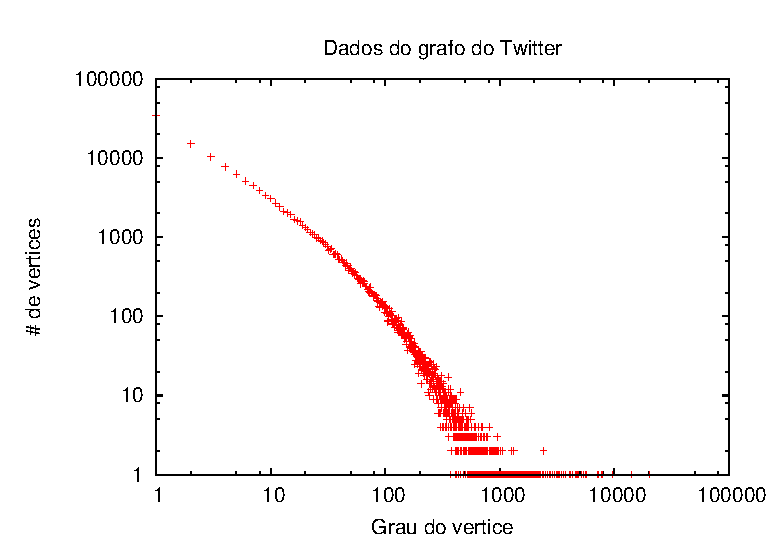
\includegraphics[width=0.7\linewidth]{power_law.eps}}
	\caption{Distribuição de dados de redes sociais (\emph{power-law}) com dados do Twitter}
	\label{fig:powerlaw}
\end{figure}

Nos exemplos que iremos demonstrar durante a execução deste minicurso, serão utilizados dois conjuntos
de dados, que foram utilizados por Leskovec et al. \cite{leskovec2012learning} e encontram-se 
disponibilizados pelo Projeto SNAP (\textit{Stanford Network Analyst Project}), contendo
usuários do Facebook e do Twitter, com estatísticas descritas na Tabela \ref{tab:datasets}.
Deve-se atentar para o fato de que o Twitter e o Facebook possuem políticas diferentes; no Twitter
é possível que um usuário siga algum outro sem que este também o siga de volta, enquanto que
no Facebook a contrapartida é exigida. Isto torna o grafo do Twitter direcionado e o do Facebook
não direcionado. Nós iremos, nos nossos exemplos, lidar com grafos direcionados e, portanto, será
necessário duplicar os dados do Facebook, criando a volta de cada ligação ou aresta.

\begin{table}[!htbp]
\caption{Estatísticas dos conjuntos de redes sociais (Facebook e Twitter) utilizados.}
\centering
\begin{tabular}{l|l|l}
\hline
\hline
Conjunto de dados & Facebook & Twitter \\
\hline
\hline
Vértices          & 4.039     & 81.306 \\
\hline
Arestas           & 88.234    & 1.768.149 \\
\hline
Triângulos        & 1.612.010 & 13.082.506 \\
\hline
\hline
\end{tabular}
\end{table}



\section{Bancos de dados relacionais}
\label{sec:relacional}

Bancos de dados relacionais são sistemas que implementam o modelo de dados
relacional proposto por Codd na década de 70 \cite{Codd1970}, rapidamente
implementado por um sistema chamado System R da IBM \cite{Astrahan1976}.
A principal ideia é a de representar os dados em forma de relações (tabelas)
e as operações são definidas a partir de uma álgebra: a álgebra relacional.
O sistema recebe comandos através de uma linguagem declarativa (SQL) 
\cite{Chamberlin1974}, os converte em operadores da álgebra relacional
para então poder ser executada nos dados persistentes nas relações.

\begin{figure}
        \centering
        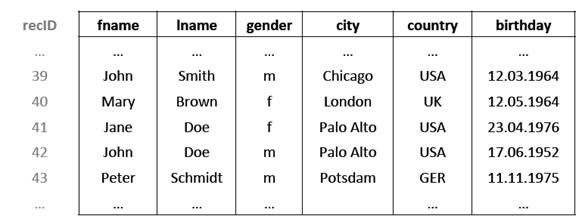
\includegraphics[width=\linewidth]{./colunar_repr_tabela.png}
        \caption{Representação de uma tabela em um banco de dados relacional.}
        \label{fig:tabular}
\end{figure}

A Figura \ref{fig:tabular} mostra a representação de uma relação contendo 
informações sobre indivíduos em um formato de tabela. Esta relação possui
os seguintes atributos do indivíduo : (i) \emph{fname}, o nome; (ii) 
\emph{lname}, o sobrenome; (iii) \emph{gender}, o sexo, \emph{m} para 
masculino e \emph{f} para feminino; (iv) \emph{city},
a cidade onde nasceu; (v) \emph{country}, o país onde nasceu; e 
(vi) \emph{birthday}, a data de nascimento.

Os principais operadores da álgebra relacional são: projeção ($\Pi$),
seleção ($\sigma$), junção ($\bowtie$). Sejam duas relações $R$ e $S$
com atributos $r_1, \ldots, r_m$ e $s_1, \ldots, s_n$, representadas
por $R(r_1, \ldots, r_m)$ e $S(s_1, \ldots, s_n)$. Uma projeção em $R$
recebe como argumento uma lista de atributos subconjunto dos atributos
de $R$ e retorna a relação contendo somente os atributos desta lista.
A projeção é representada por $\Pi_{lista~de~atributos}(R)$. Uma seleção
em $R$ recebe como argumentos uma condição em forma de predicado e 
retorna todas as tuplas em $R$ que satisfazem o predicado. A seleção 
é representada por $\sigma_{predicado} (R)$. A junção é um operador
binário e é aplicado sobre duas relações $R$ e $S$, recebe como argumento
uma condição em forma de predicado (usualmente a igualdade entre dois
atributos das relações $R$ e $S$), e retorna a relação correspondente
ao produto cartesiano das duas relações $R$ e $S$ cujas tuplas satisfazem
o predicado da junção. A junção é representada por $R \bowtie_{predicado} S$. 

A linguagem SQL expressa de forma declarativa operações sobre os dados
armazenados nas relações a partir da álgebra relacional. Uma versão simplificada
da linguagem SQL é mostrada a seguir:

\begin{lstlisting}[style=MySQLStyle]
SELECT <lista de atributos>
FROM   <lista de tabelas>
WHERE  <predicado>;
\end{lstlisting}

Após o sistema receber uma consulta na linguagem SQL, esta deve ser expressada
segundo operadores da álgebra relacional da forma mais eficiente possível. Um 
otimizador de consultas é o responsável por esta tradução. A ordem dos operadores
influencia no resultado; normalmente seleções ($\sigma$) são as primeiras a serem
executadas, pois reduzem o tamanho das relações resultantes. A ordem das junções
também é de extrema importância; uma junção entre as relações $R$, $S$ e $T$ pode
ser executada nas seguintes ordens: (i) $R \bowtie S \bowtie T$, (ii) 
$R \bowtie T \bowtie S$ e (iii) $S \bowtie T \bowtie R$. Adicionalmente, existem
inúmeros algoritmos para a execução eficiente das junções que devem coexistir no
sistema e serem utilizados em circunstâncias em que são os mais eficientes 
\cite{Mishra1992}.

O problema da contagem de triângulos da Seção \ref{sec:triangulos} pode ser expresso na 
seguinte consulta SQL, assumindo que temos uma relação chamada Twitter com os attributos
\emph{follower} e \emph{followee} contendo números inteiros de identificadores de usuários
representando relacionamentos na rede social, onde \emph{follower} segue \emph{followee}.

\begin{lstlisting}[style=MySQLStyle]
SELECT COUNT(*) 
FROM   TWITTER R, TWITTER, S, TWITTER T
WHERE  R.followee = S.follower AND
       S.followee = T.follower AND
       T.followee = R.follower AND
       R.follower > S.follower AND
       S.follower > T.follower;
\end{lstlisting}

Uma forma de execução desta consulta, em operadores da álgebra relacional é 
\begin{multline}
\sigma_{S.follower > T.follower}(\sigma_{R.follower > S.follower}(( R \bowtie_{R.followee = S.follower} S ) \\
\bowtie_{(S.followee = T.follower) \land (T.followee = R.follower)} T))
\end{multline}

Este plano de execução irá seguir os seguintes passos:

\begin{enumerate}
\item Primeira junção entre as tabelas $R$ e $S$ com predicado $R.followee = S.follower$
\item Seleção com predicado $R.follower > S.follower$ aplicado ao resultado anterior
\item Junção do resultado anterior com a tabela $T$ com predicado $(S.followee = T.follower) \land (T.followee = R.follower)$
\item Seleção com predicado $S.follower > T.follower$
\end{enumerate}

Os principais players deste mercado de bancos de dados relacionais são Oracle Database, Microsoft 
SQL Server, IBM DB2 e os de código aberto MySQL e PostgreSQL. 


\section{Bancos de dados colunares} 
\label{sec:colunar}

A ideia por traz dos bancos de dados colunares não é nova. Uma das primeiras propostas de organizar os 
dados de um banco de dados por colunas, em vez da tradicional representação por linhas dos bancos de 
dados relacionais, apareceu em 1969 \cite{Estabrook1969327}. De forma resumida, enquanto um banco de 
dados relacional tradicional armazena cada registro ou tupla em um espaço contínuo do disco (ou memória), 
os bancos de dados colunares armazenam cada coluna em espaços contínuos \cite{Abadi2009}. 

A grande vantagem da representação colunar é a compressão de dados, uma vez que o domínio dos dados 
é preservado em espaços contíguos de disco ou memória. 
Uma das principais formas de compressão de dados é por dicionário, onde cada coluna de uma 
tabela (ou relação) é dividia em um índice com os valores distintos ordenados e um vetor com a 
codificação dos valores de cada tupla na mesma sequência em que aparecem na tabela. 
Esta codificação utiliza um numero mínimo de bits do domínio de valores de cada registro, 
baseada no dicionário. Com os dados comprimidos, menos Bytes trafegam entre o disco e a 
memória principal, tornando operações de consulta e agregação mais rápidas.
A Figura \ref{fig:tabular} mostra a representação tradicional de uma tabela num banco de dados 
relacional tradicional (orientado por linhas) e a Figura \ref{fig:colunar} mostra como a 
primeira coluna da relação é organizada em um banco de dados colunar.

\begin{figure}
	\centering
	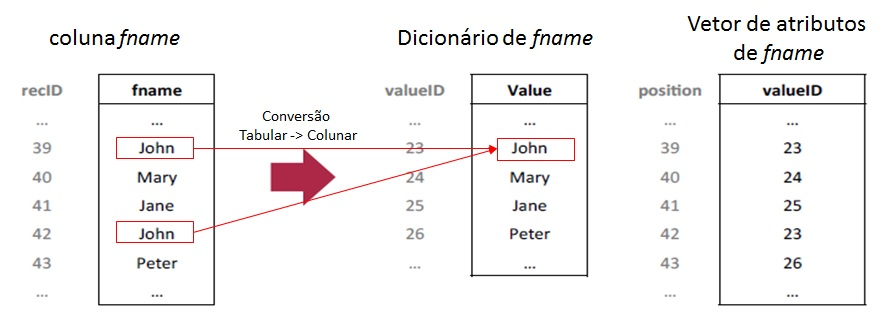
\includegraphics[width=\linewidth]{./Representacao_colunar.jpg}
	\caption{Organização da coluna fname em um banco de dados colunar.}
	\label{fig:colunar}
\end{figure}


Para explicar melhor o mecanismo de compressão, imaginemos que a coluna \textbf{fname} tenha 
100 caracteres representados por 1 Byte cada. Imaginemos também que a tabela em questão trata-se 
da lista de todos os cidadãos brasileiros, ou seja, teremos aproximadamente 200 milhões de registros. 
Logo, o espaço de armazenamento no modelo tradicional é de $200*10^6 * 100~Bytes \cong 18,62~GBytes$. 
No armazenamento em formato de colunas, os dados são armazenados em um dicionário que contém uma 
entrada para cada valor distinto. Imaginemos que há 10 mil nomes (primeiro nome) distintos no Brasil. 
Com isso, para o dicionário, precisamos de $10*10^3 * 100~Bytes \cong 1~MByte$. Já o vetor de 
valores conterá os 200 milhões de registros, mas codificados pela quantidade mínima de bits 
necessários para se codificar os 10 mil valores distintos $log_2 10.000 \cong 13,2$, ou seja, 
14 bits. Nesse caso, o vetor de valores terá $200*10^6 * 14~bits \cong 2,6~GBytes$. Nesse simples 
exemplo, podemos observar um fator de compressão de $18,62 / (0,001 + 2,6) \cong 7,2$ vezes.

A recuperação de um determinado registro (tupla) passa por um acesso direto à posição dele em 
cada uma dos vetores de valor das colunas da tabela e mais um acesso em cada dicionário para traduzir 
a codificação no valor original.

O grande problema nessa representação são operações de remoção e inserção, que usualmente causam uma 
reorganização do dicionário e consequentemente uma reorganização de todos os dados da coluna cujo 
dicionário foi reordenado. Por isso, o uso desse tipo de tecnologia deve ser preferível em conjuntos 
de dados cuja operação predominante seja de consulta. Plattner \cite{plattner2009common} alega que 
os bancos de dados corporativos possuem uma carga predominantemente de consulta e com isso, 
pode-se unificar os repositórios OLTP e OLAP na mesma estrutura. 

Os sistemas modernos que utilizam a representação colunar lançam mão de diversas estratégias para 
minimizar esses efeitos de reorganização dos dicionários. O SAP HANA, por exemplo, divide os dados 
em principal e diferencial \cite{plattner2012memory}. Novos registros e atualizações de valores são 
incluídos no conjunto diferencial, que é mantido em tamanho pequeno. As operações de consulta juntam 
os dados do conjunto principal com o conjunto diferencial. Embora a busca no conjunto diferencial seja 
ineficiente, ela é realizada sobre um conjunto pequeno de dados. De tempos em tempos, os conjuntos são 
mesclados resultando em um novo conjunto principal e um conjunto diferencial praticamente vazio, que 
conterá apenas as operações realizadas durante a operação de mesclagem.

Há também outros mecanismos de compressão para outros domínios de dados, e.g. números inteiros e de ponto 
flutuante \cite{Abadi2006, Zukowski2006}. É importante ressaltar que todos estes mecanismos de 
compressão de dados tentam balancear a taxa de compressão de dados com o processamento para compressão
e descompressão; em geral, os mecanismos mais eficientes em termos de taxa de compressão não são utilizados,
uma vez que o processamento (CPU) para descompressão dos dados durante a execução das consultas
pode ser um fator determinante. Adicionalmente, em geral, todos os mecanismos de compressão de dados
preservam as propriedades de igualdade e ordenação dos dados, i.e. valores $=$, $<$ ou $>$ no domínio original
dos dados são também $=$, $<$ ou $>$ no domínio de compressão. Esta propriedade é extremamente importante, 
pois a execução de diversos algoritmos da álgebra relacional que envolvem a comparação e ordenação dos
dados, e.g. junção, podem ser executados no domínio dos dados comprimidos, evitando assim processamento 
desnecessário de descompressão dos dados. É fácil observar esta propriedade no exemplo acima da compressão
da coluna \emph{fname}, desde que o dicionário esteja ordenado por nome.

Atualmente, os principais fornecedores de bancos de dados relacionais tradicionais também fornecem 
soluções de armazenamento colunar, como Microsoft, Oracle, IBM, SAP e outros.  


\section{Bancos de dados em memória}

Sistemas de banco de dados em memória são aqueles em que a fonte primária dos dados reside 
em memória principal (RAM). Esses dados têm, usualmente, cópia em disco, para eventuais falhas 
no hardware ou simplesmente falta de energia. Embora os sistemas de bancos de dados tradicionais 
também mantêm algum dado em memória como forma de fazer \textit{cache}, a principal diferença é 
que, nos bancos de dados em memória, a fonte de dado primária (ou principal) está 
armazenada na memória RAM, enquanto nos tradicionais, está armazenada em disco \cite{garcia1992main}.

Esse tipo de tecnologia ganhou força nos últimos anos devido aos avanços nas arquiteturas de 
hardware que, atualmente, permitem sistemas com Terabytes de memória RAM compartilhadas entre 
vários processadores. Além disso, houve um barateamento enorme no custo desses equipamentos, o 
que tornou viável os sistemas de banco de dados em memória. 

Como o acesso à memória principal chega a ser cerca de 1.000 vezes mais rápido que os discos modernos 
como SSD (disco de estádo sólido), esse tipo de tecnologia é bem convidativo. O leitor mais atento 
pode se perguntar: e se um sistema de banco de dados tradicional tiver um \textit{cache} grande o 
suficiente para caber todo o volume de dados, qual seria a diferença? Ainda sim esses sistemas são 
projetados de forma não ótima para uso da memória, pois há ainda a indireção do \textit{cache}. 
Por exemplo, será necessário consultar um gerenciador do \textit{cache} toda vez que for acessar o dado;
outro exemplo são as estruturas dos índices, que estão em estruturas onde o acesso não é imediato (Árvores B+). 

Embora existam hardwares especializados com memória não volátil, fontes de energia redundantes e 
outros mecanismos para minimizar falhas no hardware, ainda é virtualmente impossível garantir que o 
dado em memória principal esteja seguro. Por isso, uma questão muito importante para bancos de dados 
em memória é a recuperação de falhas. Em bancos de dados em memória, a estratégia tipicamente utilizada 
é persistir em disco cada uma das transações em um \textit{log}. Uma transação só é concluída após a 
escrita da mesma no disco (\textit{log}). De tempos em tempos, são criados \textit{checkpoints}, onde 
uma cópia da memória principal é realizada em disco, podendo descartar os \textit{logs} de transações 
anteriores ao \textit{checkpoint}. A frequência da criação desses \textit{checkpoints} depende da 
confiabilidade do hardware e da volatilidade dos dados.

Outras questões importantes do projeto de sistemas de bancos de dados em memória, como controle de concorrência, processamento de transações, organização dos dados, métodos de acesso, processamento de consultas, desempenho e clusterização são discutidos em mais detalhes por Garcia-Molina e Salem \cite{garcia1992main}.

Atualmente, praticamente todos os grandes fornecedores de soluções tradicionais de bancos de dados 
relacionais também possuem versões em memória de seus produtos, como Microsoft, Oracle e IBM, mas 
também há fornecedores especializados nesse tipo de solução. Alguns desses produtos também possuem 
características de bancos de dados colunares (Seção \ref{sec:colunar}, principalmente com o objetivo 
de atingir boa compressão dos dados e melhor utilização da memória.






\section{Bancos de dados paralelos}

Bancos de dados paralelos ou massivamente paralelos (MPP, do inglês 
\emph{massively parallel processing}) também não são tecnologia 
recente, discussões sobre esse assunto e implementações de sistemas
datam da década de 80-90 \cite{Dewitt1992, Fushimi1986}. Nestes 
sistemas, os dados das tabelas são distribuídos em diversos 
nós de um cluster e o processamento de consulta é paralelizado.

Os dados podem ser distribuídos através de particionamento vertical,
onde as tabelas são quebradas por colunas; horizontal, onde as 
tabelas são quebradas por tuplas; ou ambos. A distribuição dos 
dados entre os nós pode utilizar o conhecimento prévio
das consultas mais utilizas no sistema (\emph{query workload}),
e o otimizador de consultas, nestes casos, conhecendo a forma
como os dados estão distribuídos, pode repassar a parte das
consultas para os nós específicos que devem processá-la. O problema
geral desta abordagem é que existe a possibilidade de desbalanceamento
de nós \emph{data skew}; e o particionamento por funções de hash é portanto também
bastante utilizado, pois através de boas funções de hash é possível
evitar este desbalanceamento..

A arquitetura dos bancos de dados paralelos pode ser de compartilhamento 
de memória (\emph{shared-memory}, onde a memória é compartilhada entre os
nós do cluster; compartilhamento de disco (\emph{shared-disk}), onde
cada nó do cluster possui sua própria memória, mas o disco é compartilhado
entre todos os nós; ou sem compartilhamento (\emph{shared-nothing}), onde
cada nó possui sua própria memória e disco e o compartilhamento de dados
entre nós do cluster se faz através de transferência por mensagens. As 
arquiteturas com compartilhamento (\emph{shared-memory} e \emph{shared-disk})
se mostraram ineficientes em escalabilidade para grandes implantações
\cite{Dewitt1992, Stonebraker1986}. A Figura \ref{fig:mpp_arq} mostra
um banco de dados paralelo com um nó mestre e arquitetura sem 
compartilhamento.


\begin{figure}
        \centering
        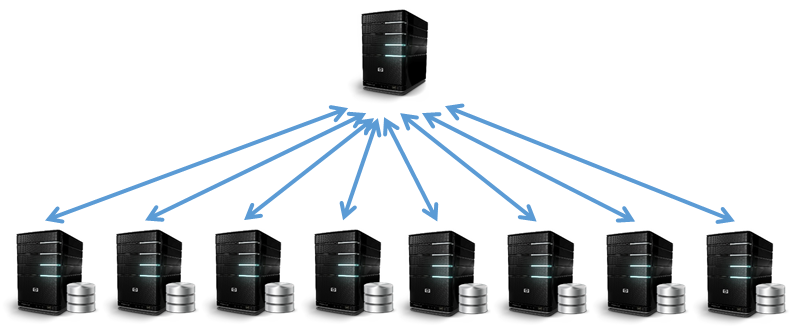
\includegraphics[width=\linewidth]{./mpp_database.png}
        \caption{Banco de dados paralelo e a arquitetura sem compartilhamento.}
        \label{fig:mpp_arq}
\end{figure}

Os operadores da álgebra relacional são todos paralelizáveis, principalmente
a junção, com algoritmos de espalhamento dos dados por função de hash 
\cite{Schneider1989}. A ideia principal destes algoritmos é a de que cada 
nó lê sua parcela dos dados, aplica uma função de hash nos atributos da
junção para determinar o nó de destino e envia os dados para os nós específicos.
Desta forma, quando os nós agora recebem os dados, há a garantia (pela
função de hash) de que os nós que irão participar do resultado da junção 
estão fisicamente localizados juntos, neste passo. Cada nó então executa um
algoritmo linear de junção, tipicamente uma junção por hash em memória,
e reporta o resultado para o nó coletor. Este processo é demonstrado na 
Figura \ref{fig:mpp_hashjoin}. Nesta figura, é mostrada uma arquitetura
com quatro nós sem compartilhamento, e estes quatro nós estão replicados 
em duas camadas para melhor mostrar a fase de espalhamento dos dados
por função de hash (\emph{shuffle}).

\begin{figure}
        \centering
        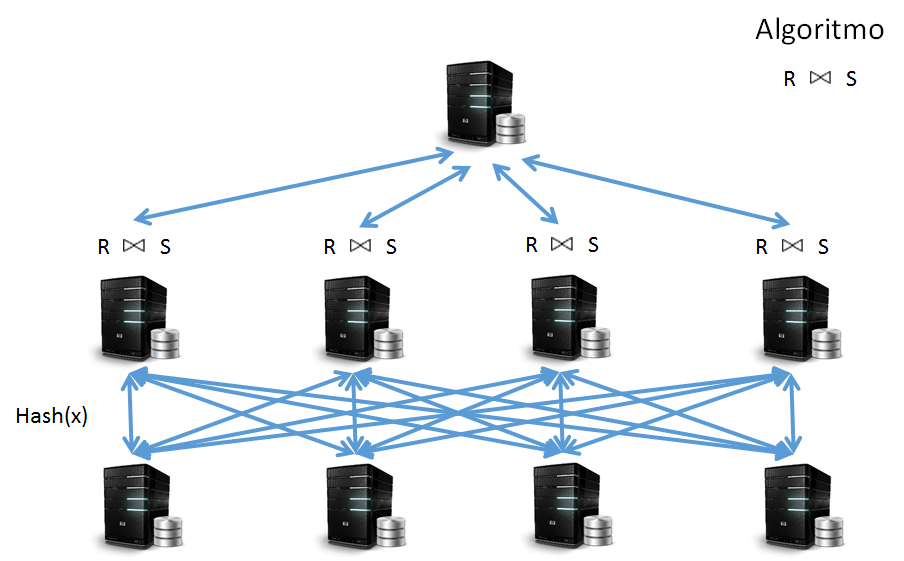
\includegraphics[width=\linewidth]{./mpp_hashjoin.png}
        \caption{Junção por hash em um banco de dados paralelo sem compartilhamento.}
        \label{fig:mpp_hashjoin}
\end{figure}

A solução do problema da contagem dos triângulos da Seção \ref{sec:triangulos} utilizando
banco de dados paralelos não envolve mistérios, uma vez que tal tecnologia 
implementa a álgebra relacional e já mostramos na Seção \ref{sec:relacional}
a consulta SQL que resolve o problema. Esta consulta envolve duas junções, 
que serão executadas em paralelo, e as seleções de remoção de duplicatas que
serão aplicadas após as junções no fluxo de execução das consultas (\emph{pipeline}).



\section{Hadoop}
\subsection{Breve histórico}
O problema era simples: como criar um índice para uma máquina de busca de toda a Internet? Foi com esse desafio que Mike Cafarella e Doug Cutting resolveram desenvolver o Apache Nutch. Rapidamente o \textit{crawler} e a máquina de busca ficaram prontos, mas eles perceberam que a arquitetura não escalaria para criar um índice de mais de um bilhão de páginas da Internet. Na mesma época, a equipe do Google publicou um conhecido artigo que explicava a arquitetura do GFS (Google FileSystem) \cite{ghemawat2003google}, que era um sistema de arquivos distribuído que era usado em sua máquina de busca. Doug e Mike decidiram criar uma implementação \textit{open source} dessa arquitetura e a chamaram de NDFS (Nutch Distributed FileSystem).

Em 2004, a equipe do Google publicou um artigo detalhando como era possível criar um índice de toda a Internet usando um conceito denominado MapReduce \cite{dean2008mapreduce}. Com base nesse trabalho, os desenvolvedores do Nutch migraram a maior parte de seus algoritmos para executar sobre o MapReduce e o NDFS. Mais tarde, Doug Cutting foi trabalhar no Yahoo! liderando uma equipe que construiu a nova geração de máquina de busca deles. Depois, o NDFS e o MapReduce tornaram-se um projeto da Apache sob o nome de Apache Hadoop.

Desde então, o Hadoop tem sido usado mundialmente para processar enormes quantidades de dados. Vários frameworks foram construídos para executar usando a sua infraestrutura, como veremos a seguir. Diversos fornecedores criaram suas próprias distribuições do Hadoop, como Microsoft, IBM, EMC, Oracle e outras empresas especializadas como Cloudera e Hortonworks.

\subsection{Funcionamento do HDFS}
O HDFS, como mencionado acima, é um sistema de arquivos distribuídos, projetado para armazenar arquivos muito grandes\footnote{Atualmente há instâncias do HDFS armazenando PetaBytes de dados.} executando sobre \textit{hardware} barato. 

Assim como em qualquer sistema de arquivos, um arquivo é dividido em \textbf{blocos} de dados. Enquanto, tipicamente um sistema de arquivos tradicional armazena dados em blocos de 512 bytes, o HDFS usa, por padrão, blocos de 64MB. Isso torna o HDFS ineficiente para uso em arquivos muito pequenos e numerosos. Para garantir disponibilidade e leitura em paralelo, cada um dos blocos é replicado em um dos nós de um \textit{cluster} HDFS. Quando um disco ou um dos nós do \textit{cluster} falha, além do bloco poder ser lido de outro nó, o sistema de arquivos automaticamente recria os blocos presentes naquele disco em outros nós do \textit{cluster}.
\begin{figure}
	\centering
	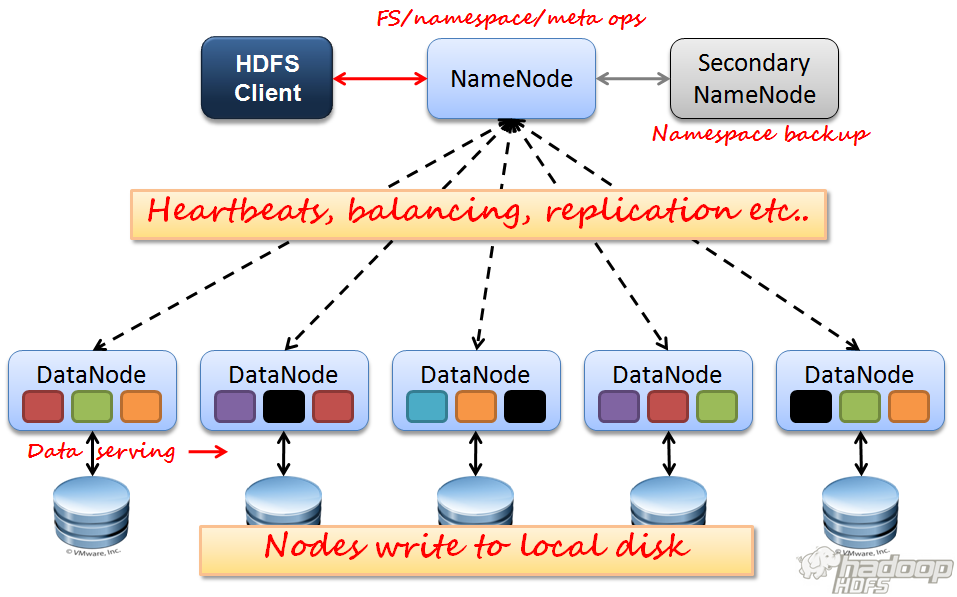
\includegraphics[width=\linewidth]{./hdfs_architecture.png}
	\caption{Visão geral da arquitetura do HDFS}
	\label{fig:hdfs_arch}
\end{figure}

A arquitetura de um \textit{cluster} HDFS divide-se em \textit{NameNode} e \textit{DataNode}. O primeiro armazena um índice de arquivos e de seus blocos e o segundo armazena os dados (blocos). Um cliente que queira ler arquivos no HDFS, primeiro consulta o \textit{NameNode}, que então diz de quais nós do cluster os blocos serão lidos, garantindo um balanceamento de carga na leitura. Arquivos criados no HDFS só podem ser modificados anexando conteúdo no final. Não pode-se modificar blocos já escritos. A falha do \textit{DataNode} implica na indisponibilidade de todo o HDFS e, por esse motivo, é importante mantê-lo resiliente a falha com mecanismos de redundância. Uma visão geral dessa arquitetura pode ser vista na figura \ref{fig:hdfs_arch}.

\subsection{O ecossistema Hadoop}
Atualmente o Hadoop conta com um ecossistema com diversos \textit{frameworks}. Uma lista, não exaustiva, de alguns dos principais projetos que compõem o ecossistema pode ser vista abaixo.
\begin{itemize}
	\item Ambari: Uma ferramenta web para aprovisionamento e gerenciamento de um cluster Hadoop e de diversos de seus componentes.
	\item HBase: Um banco de dados relacional e colunar que utiliza a infraestrutura do Hadoop como mecanismo de armazenamento.
	\item Hive: Uma infraestrutura de armazém de dados com suporte a sumarização de dados e consultas.
	\item Pig: Uma linguagem de alto nível para fluxo de dados e um \textit{framework} de execução de computação distribuída. 
	\item Spark: Uma \textit{engine} rápida e de propósito geral para processamento de dados em memória baseados nos dados do HDFS. O Spark oferece um modelo de programação simples e poderoso para executar uma enorme gama de atividades como ETL, aprendizagem de máquina, processamento contínuo de dados, processamento de grafos, etc.
	\item Sqoop: uma ferramenta para transferência massiva de dados entre bancos de dados relacionais e o HDFS.
	\item Mahout: Um conjunto de bibliotecas para executar algoritmos de aprendizagem de máquina e mineração de dados. Os coordenadores do projeto decidiram mover a implementação dos algoritmos de MapReduce para o Spark.
\end{itemize}

\subsection{MapReduce}
O Hadoop MapReduce é um \textit{framework} para facilitar a escrita de programas de computador para processar uma enorme quantidade de dados de forma paralela, distribuída e resiliente a falhas. Os dados de entrada para um \textit{Job} MapReduce, por estarem armazenados no HDFS, são também processados de forma distribuída, aproveitando dos dados disponíveis localmente em um nó do \textit{cluster}. Na \ref{fig:mapreduce} podemos ver um desenho esquemático de um \textit{Job} MapReduce, que  é, de forma resumida, composto por duas fases:
\begin{enumerate}
	\item Map - quando os dados são processados e produzem saídas como tuplas no formato (Chave, Valor); 
	\item Reduce - quando as tuplas com mesma chave são agrupadas para alguma atividade de agregação.  
\end{enumerate}

\begin{figure}
	\centering
	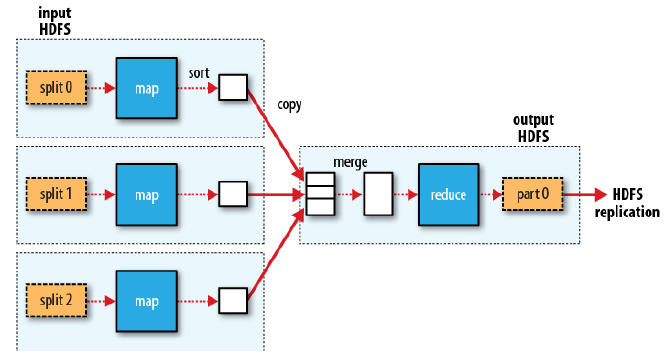
\includegraphics[width=\linewidth]{./mapreduce_job.png}
	\caption{Um \textit{Job} MapReduce}
	\label{fig:mapreduce}
\end{figure}

Um exemplo bem simples para entender o MapReduce é um Job para contar a ocorrência de cada palavra em um texto. Na fase de Map, cada linha lida do arquivo é dividida em suas palavras que produzem uma saída (PalavraA, 1). Note que se uma palavra aparece duas vezes na mesma linha duas tuplas idênticas serão produzidas. Na faze de Reduce, as tuplas com mesma chave serão agrupadas e os valores serão somados. 

Em geral, o programador não precisa se preocupar com comunicação de dados, tratamento de concorrência e eventuais falhas em algum nó que está processando um determinado \textit{Job}. Esse é um dos grandes diferenciais do Hadoop MapReduce. 

\subsection{Pig}
nessa seção vou explicar o mapreduce e como resolver o problema do triangulo

\section{Apache Spark}
O Apache Spark é uma plataforma para computação distribuída que foi projetada para ser de propósito geral e muito eficiente \cite{karau2015learning}. A principal diferença em relação ao MapReduce é que toda a computação é feita e armazenada em memória, sem necessidade de salvar em disco resultados intermediários. 

A unidade básica de dados do Spark é o \textit{Resilient Distributed Dataset} (RDD). O conceito é semelhante ao bloco de dados do HDFS, mas trata-se de coleções de dados que estão na memória RAM dos nós do \textit{cluster}. Na prática, o Spark carrega os dados de um bloco do HDFS na memória RAM do nó em que o bloco está. Os programas Spark fazem dois tipos de operação com um RDD:
\begin{itemize}
	\item \textbf{Transformações}: Transformam um RDD em outro RDD. Entre as transformações mais comuns podemos encontrar as operações de Map e ReduceByKey (mesmo conceito do MapReduce), ordenação e operações de conjuntos, como união, interseção e diferença.
	\item \textbf{Ações}: Produzem algum resultado a partir de um RDD. Ações típicas consistem em enumerar alguma quantidade de itens de um RDD, contar e somar. 
\end{itemize}

O Spark utiliza o conceito de "execução preguiçosa", para que só quando realmente um resultado tenha de ser produzido (uma \textbf{ação} é executada), e toda a sequência de passos necessária é conhecida, o Spark realmente lê os dados e faz cálculos na memória. Com isso, o motor de execução do Spark consegue otimizar tudo que será executado, escolhendo os melhores nós, a melhor sequência, etc.

O Apache Spark também vem com um conjunto de bibliotecas com algoritmos para aprendizado de máquina, grafos, fluxo contínuo de dados e SQL. Algumas dessas vermos a seguir.

\subsection{Utilizando o console python}
O Apache Spark possui consoles iterativos nas linguagens Python e Scala e seus \textit{Jobs} podem ser submetidos em batch também em Java. A API do Spark é acessada a partir de um objeto central denominado \texttt{ SparkContext }. Esse objeto contém a conexão com uma instância do cluster e a partir dele todos os outros objetos e métodos são acessados. Ao se iniciar um console do Spark, o objeto já está automaticamente disponível através da variável \texttt{ sc }. Para compreender a simplicidade do modelo de programação do Spark, o trecho de código abaixo lê um arquivo txt e faz a contagem de ocorrência das palavras.

\begin{lstlisting}[style=MyPythonStyle]
    ##produz um RDD onde cada item e uma linha do arquivo texto
    arquivo = sc.textFile('hdfs://servidor:10001/arquivo.txt') 
    ##para cada linha produz N itens no novo RDD, uma para cada palavra.
    palavras = arquivo.flatMap(lambda linha : linha.split(' ')) 
    ##cria novo RDD com tuplas do formato (palavra, 1)
    palavrasCV = palavras.map(lambda palavra : (palavra, 1)) 
    ##executa o Reduce usando a funcaoo add para os valores das tuplas.
    contagemPalafras = palavrasCV.reduceByKey(add) 
    ##somente nesse comando toda a computacaoo e feita de forma otimizada.
    contagemPalavras.collect() 
\end{lstlisting}

Para resolver o problema de contagem de triângulos utilizando o Spark, a idéia é semelhante à usada com o modelo do MapReduce.

\subsection{Spark SQL}
O Spark SQL é um módulo do Apache Spark para processamento de dados estruturados (relacionais). Ele utiliza uma abstração denominada DataFrame, e também serve como uma máquina de execução de consultas distribuídas baseada em SQL. 

Um DataFrame do Spark SQL tem as mesmas características de um DataFrame em R ou em Pandas (Python) e pode ser criado baseando-se em diversas fontes de dados, como um arquivo json, um arquivo texto, um RDD do Spark, uma tabela do Hive, ou qualquer fonte que possua um driver JDBC. O \textit{schema} de um DataFrame pode ser inferido através de reflexão ou definido programaticamente. 

O trecho de código abaixo mostra como executar a contagem de triângulos utilizando o SQL proposto na seção \ref{triangulos}.

\subsection{Spark GraphX}
O Spark GraphX é um novo módulo do Apache Spark que fornece um conjunto de abstrações e ferramentas para processamento paralelo de grafos. Nas abstrações de nós e arestas é possível incluir propriedades, como pesos, capacidades máximas e mínimas, ou qualquer outra propriedade que seja relevante para modelar um problema. 

O Spark GraphX possui um conjunto de operações essenciais para diversos algoritmos de análise de grafos, como operações em paralelo sobre os nós/arcos dos grafos, obtenção de subgrafos, inversão de arestas e agregação de vizinhos. Esse último, por exemplo, pode ser usado para calcular o grau de cada vértice de um grafo. Mais detalhes desse módulo podem ser obtidos na documentação oficial do produto \footnote{http://spark.apache.org/docs/latest/graphx-programming-guide.html}. 

Como é recente seu desenvolvimento, ainda são poucos os algoritmos implementados e a única linguagem suportada é o Scala. Atualmente conta com algoritmos de PageRank, Identificação de componentes conectados e contagem de triângulos, que demonstramos o uso no trecho de código abaixo. Comparado com as estratégias de MapReduce, a contagem de triângulos utilizando Spark GraphX é de várias ordens de grandeza mais rápido e eficiente em consumo de memória. 

\begin{lstlisting}[style=MyPythonStyle]
    ## Carrega o grafo a partir de um arquivo cujas linhas sao pares de identificadores dos nos, definindo uma aresta
    val graph = GraphLoader.edgeListFile(sc, "graphx/data/followers.txt", true).partitionBy(PartitionStrategy.RandomVertexCut)
    ## conta o numero de triangulos
    val triCounts = graph.triangleCount().vertices
    ## imprime o resultado
    println(triCounts.mkString("\n"))
\end{lstlisting}

\section{Considerações finais}

column-store vs row-store \cite{Abadi2008}

vários \cite{Pavlo2009}

Hadoop vs banco de dados paralelo \cite{Stonebraker2010}

Survey of nosql \cite{han2011survey}. Comparação entre SQL e NoSQL 
\cite{cattell2011scalable, stonebraker2010sql}

NewSQL \cite{stonebraker2012newsql}. Anti-caching \cite{debrabant2013anti}


% you should really use BibTeX instead of this... :-)
\bibliographystyle{dinat}
\bibliography{bibliografia}


\end{document}
